	%\newpage
	\section{Measurement of Semiconductors}
	The currentflow of the device with currentless control gate (third pin, also called Tristate pin)
is to be examined first.
The Tristate pin of the device under test is the base or gate for example.
One probe pin is selected as the positive side of the device and connected directly to VCC.
The other probe pin  selectes as negative side of the device.
The negative side is connected with the \(680~\Omega\) resistor to GND.
With fieldeffect transistors the state of the device depends on the voltage of the gate.
The Tristate pin is first connected with the \(680~\Omega\) resistor for \(5~ms\) to the GND side and
the voltage at the negative side is measured.
After that the voltage of the negative side is measured again during the Tristate pin switched
as input (High Impedance).
Then the assumed gate is connected with the \(680~\Omega\) resistor for \(5~ms\) to the VCC side and
the voltage on the negative side is measured again.
If the measured voltage is lower than the first measurement result, this circuit will
be assumed as the right one. Then the voltage is measured again with currentless Tristate pin.

If the voltage of the negative pin with fixed Tristate pin is higher than \(115~mV\) and
this level is not \(100~mV\) lower than the voltage measured with currentless Tristatepin,
a depletion transistor type is assumed.
With bipolar transistors, which have a high collector residual current,
the residual current with currentless base is usually significant higher.
With the checking of both voltages we can avoid the wrong detection of some Germanium transistors with a higher
collector cutoff current as depletion transistors (JFET).

Then additional tests are done 
to differ N-channel JFET or N-D-MOSFET and P-channel JFET or P-D-MOSFET.
The MOSFET versions can be differed by the missing of gate current in any state
of the TriStatePin.

To get parameters of the depletion types, they will be measured with a \(680~\Omega\) resistor at
the source pin, as shown in figure~\ref{fig:JFETcd} . This measurement will be done instead of the
usually measurement of current with the gate hold at source level, because
the \(I_\mathrm{DSS}\) current of the FET transistor can often not be reached
with the relative high resistance of the \(680~\Omega\) resistor.

\begin{figure}[H]
\centering
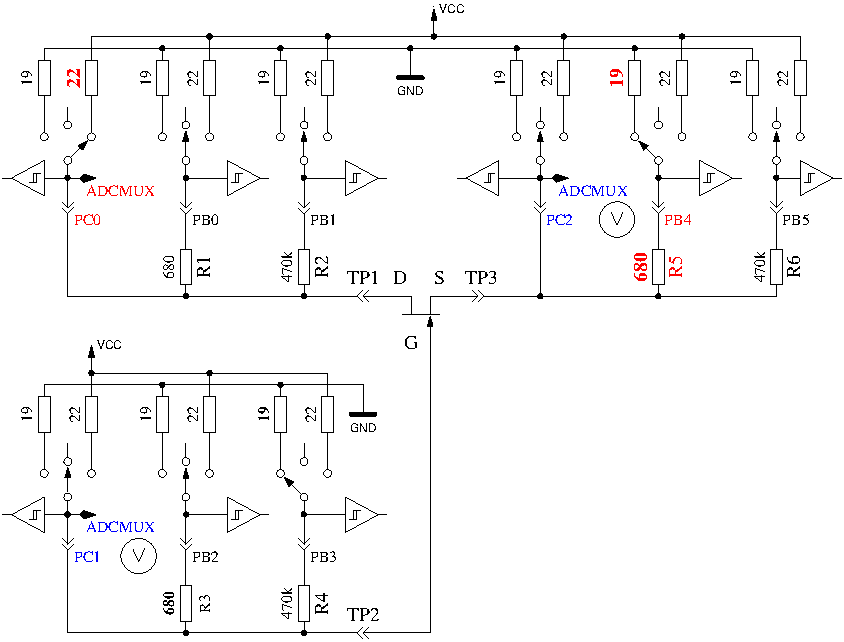
\includegraphics[width=.8\textwidth]{../FIG/JFETcd.pdf}
\caption{Measurement of the  Gate-Source voltage and Source current of a N-JFET transistor}
\label{fig:JFETcd}
\end{figure}

If the component has no current between positive probe and negative probe without signal at the
TristatePin, the next tests are specified in the next section~\ref{sec:pnp}.
If current was detected, the next test is described in the diode section~\ref{sec:diode}.

\subsection{Measurement of PNP Transistor or P-Channel-MOSFET}
\label{sec:pnp}
First the current amplification factor is measured with common collector (emitter follower) for the assumed
PNP transistor.
The measuring situation is shown in figure~\ref{fig:pnpcc}.
If the measured voltage at the Base (\(UB\)) is above \(9~mV\) with the \(680~\Omega\) resistor,
the hFE is build as \(hFE = \frac{UE-UB}{UB}\).
The voltage \(UE\) is the difference of the Emitter-voltage to VCC.
The difference between the \(22~\Omega\) and \(19~\Omega\) resistors are not respected.
If the \(UB\) voltage is below \(10~mV\), the measurement is done with the \(470~k\Omega\) resistor at the base.
In this case the current amplification factor is build as \(hFE = \frac{UE \cdot 470000}{UB \cdot (680+22)}\).

\begin{figure}[H]
\centering
 \begin{overpic}[width=1.\textwidth]{../FIG/PNPcc.pdf}
  \color{black}
   \put(55,20){\makebox(0,0)[lb]{\footnotesize {The \textcolor{green}{green} switch state is used}}}
   \put(55,17){\makebox(0,0)[lb]{\footnotesize {if Voltage at PC1 is  \textless~10mV !}}}
 \end{overpic}
\caption{hFE measurement of PNP transistor with common collector circuit }
\label{fig:pnpcc}
\end{figure}

Next the tests with common emitter are done for the assumed PNP transistor.
The positive side of component is now direct connected to VCC, the negative side \(680~\Omega\) resistor
is connected to GND as shown in Figure~\ref{fig:pnpce}. 
If the negative side of component has a voltage of above \(3.4~V\), when the base side \(680~\Omega\) resistor 
was connected to GND, it must be a PNP transistor or a P-Channel FET.
This can be easy find out by analysing the base voltage. If the base voltage is greater \(0.97~V\), it must be a PNP.
For measuring the current amplification factor, the \(470~k\Omega\) resistor is taken as Base resistor
instead of the \(680~\Omega\).
The current amplification factor is build by \(hFE = \frac{(UC-UC0) \cdot 470000}{UB \cdot (680+19)}\) .
The voltage UC0 is the voltage at the colletor resistor without base current.
The higher current amplification factor is assumed to be the right one, this one or the one found with
the common collector circuit.


The values found for the PNP are only valid, if a second
set of measurements is done.
In order to prevent detecting the PNP in the inverse mode (collector and emitter are swapped),
the measurement with the higher current amplification is taken as the right one.
If base voltage is lower than \(0.97~V\), it must be a P-E-MOS.
In this case the gate threshold voltage is measured
by switching the gate slowly with the \(470~k\Omega\) resistor up and down, waiting for a digital
input signal change of the Drain side and then read the voltage of the gate pin.

\begin{figure}[H]
\centering
 \begin{overpic}[width=1.\textwidth]{../FIG/PNPce.pdf}
  \color{black}
  \put(55,21){\makebox(0,0)[lb]{\footnotesize {The black state of switches is used for test!}}}
  \put(55,17){\makebox(0,0)[lb]{\footnotesize {The \textcolor{green}{green} state is used for current}}}
  \put(55,13){\makebox(0,0)[lb]{\footnotesize {amplification factor hFE.}}}
 \end{overpic}
\caption{test and hFE measurement of PNP transistor with common emitter circuit }
\label{fig:pnpce}
\end{figure}

\subsection{Measurement of NPN Transistor or N-Channel-MOSFET}
The measuring of NPN-Transistors begin in the same way as PNP-Transistors with measuring
the current amplification factor in the common collector circuit.
First measurement is done with a \(680~\Omega\) base resistor switched to VCC. If the
voltage at the base resistor ist too low, the \(470~k\Omega\) resistor is taken instead.
Measurement then continues with the common emitter circuit as shown in figure~\ref{fig:npnce}.

\begin{figure}[H]
\centering
 \begin{overpic}[width=1.\textwidth]{../FIG/NPNce.pdf}
  \color{black}
  \put(55,23){\makebox(0,0)[lb]{\footnotesize {The black state of switches is used for test!}}}
  \put(55,19){\makebox(0,0)[lb]{\footnotesize {The \textcolor{green}{green} state is used for current}}}
  \put(55,15){\makebox(0,0)[lb]{\footnotesize {amplification factor hFE.}}}
 \end{overpic}
\caption{test and hFE measurement of NPN transistor with common emitter circuit}
\label{fig:npnce}
\end{figure}

If the voltage of collector sinks below \(1.6~V\), when the \(680~\Omega\) base resistor is connected to VCC,
ist must be a NPN, N-Channel MOSFET or Thyristor/Triac.
With two simple tests a Thyristor or Triac can be identified.
If the gate pin resistor is connected for \(10~ms\) to GND and than made currentless, the current
at the anode should stay.
If then the anode resistor is short connected to GND and reconnected to VCC, the Thyristor should not
trigger again (no current).
Please keep in mind, that only low power Thyristors can be tested, because
the holding current of the tester can reach only \(6~mA\).
If both tests attest a Thyristor, further tests with reverse polarity are done
to exclude or confirm a Triac.

If neither Thyristor nor Triac could be confirmed, it can be a NPN or N-Channel E-MOSFET.
The Base voltage of a NPN Transistor will be near the Emitter voltage, so this type can be
identified definitely.
The current amplification factor in the common emitter circuit is build by
\(hFE = \frac{(VCC-UC-UC0)\cdot 470000}{(VCC-UB)\cdot (680+22)}\).
If the voltage of the Base or better Gate  shows, that there is no or little current, part will be a N-Channel E-MOS 
(Enhancement MOSFET).
 In this case the threshold voltage is measured by switching the Gate slowly with
the \(470~k\Omega\) resistor to VCC and GND, waiting for a digital input signal change of the Drain side and
then read the voltage of the Gate pin.
This measurement is done eleven times with ADC results accumulated as shown in Figure~\ref{fig:eleven}.
The result is multiplied by four and divided by 9 to get the voltage in mV resolution.

\begin{figure}[H]
\centering
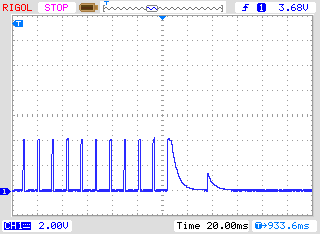
\includegraphics[width=.8\textwidth]{../PNG/IRFU120gate.png}
\caption{measuring of threshold voltage of N-Channel-MOSFET}
\label{fig:eleven}
\end{figure}

\subsection{Simplified flowchart of the transistors tests}

\begin{figure}[H]
\centering
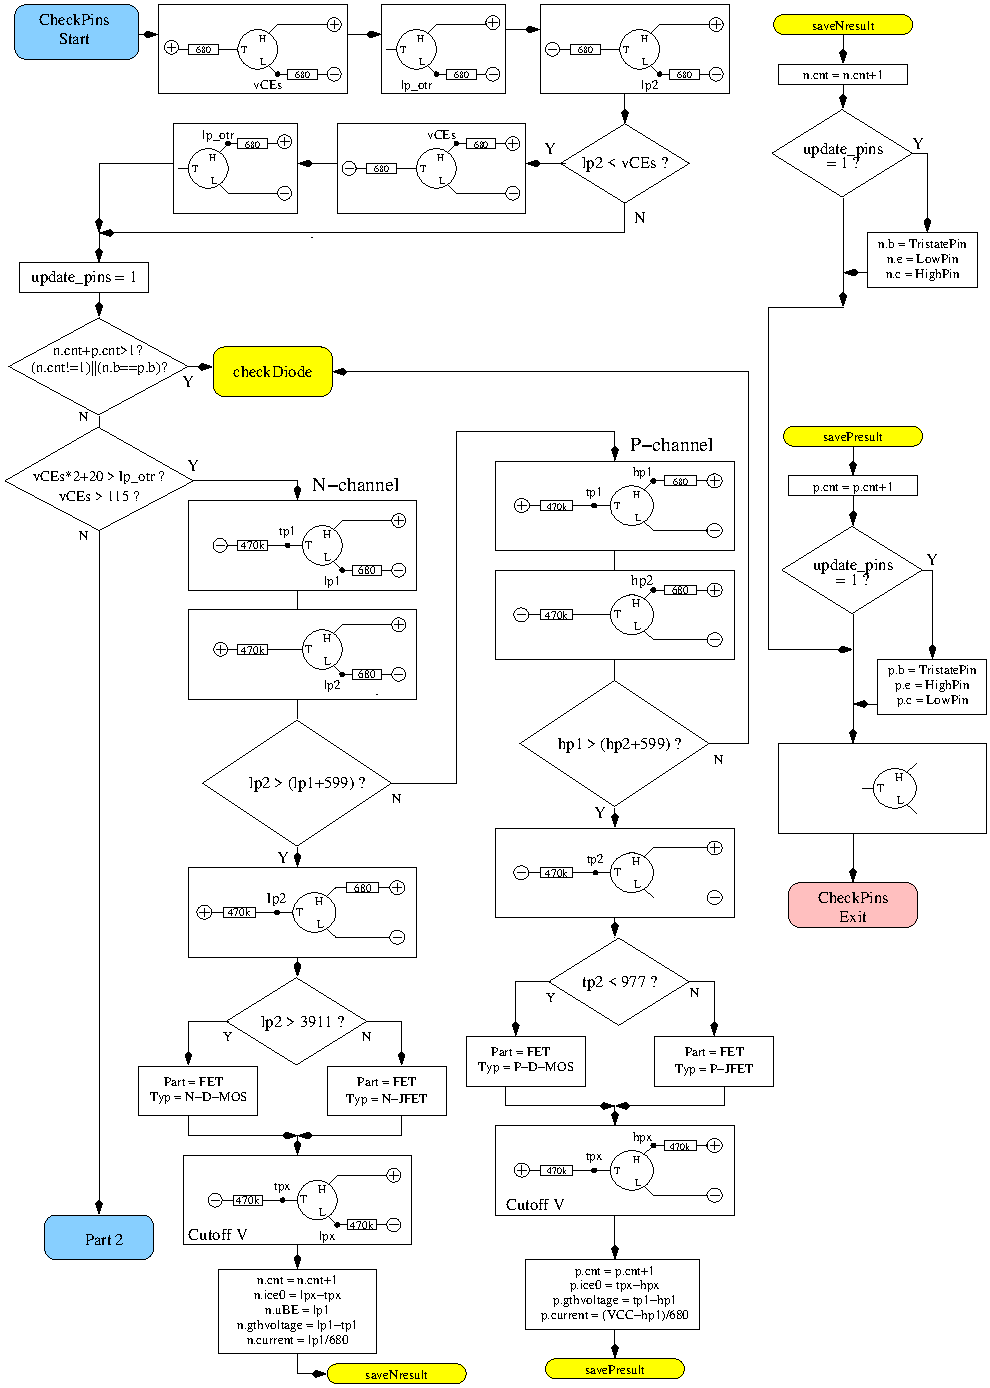
\includegraphics[width=.8\textwidth]{../FIG/CheckSemi1.pdf}
\caption{Flowchart transistor test Part 1, JFET and D-MOS}
\label{fig:ChkSemi1}
\end{figure}

\begin{figure}[H]
\centering
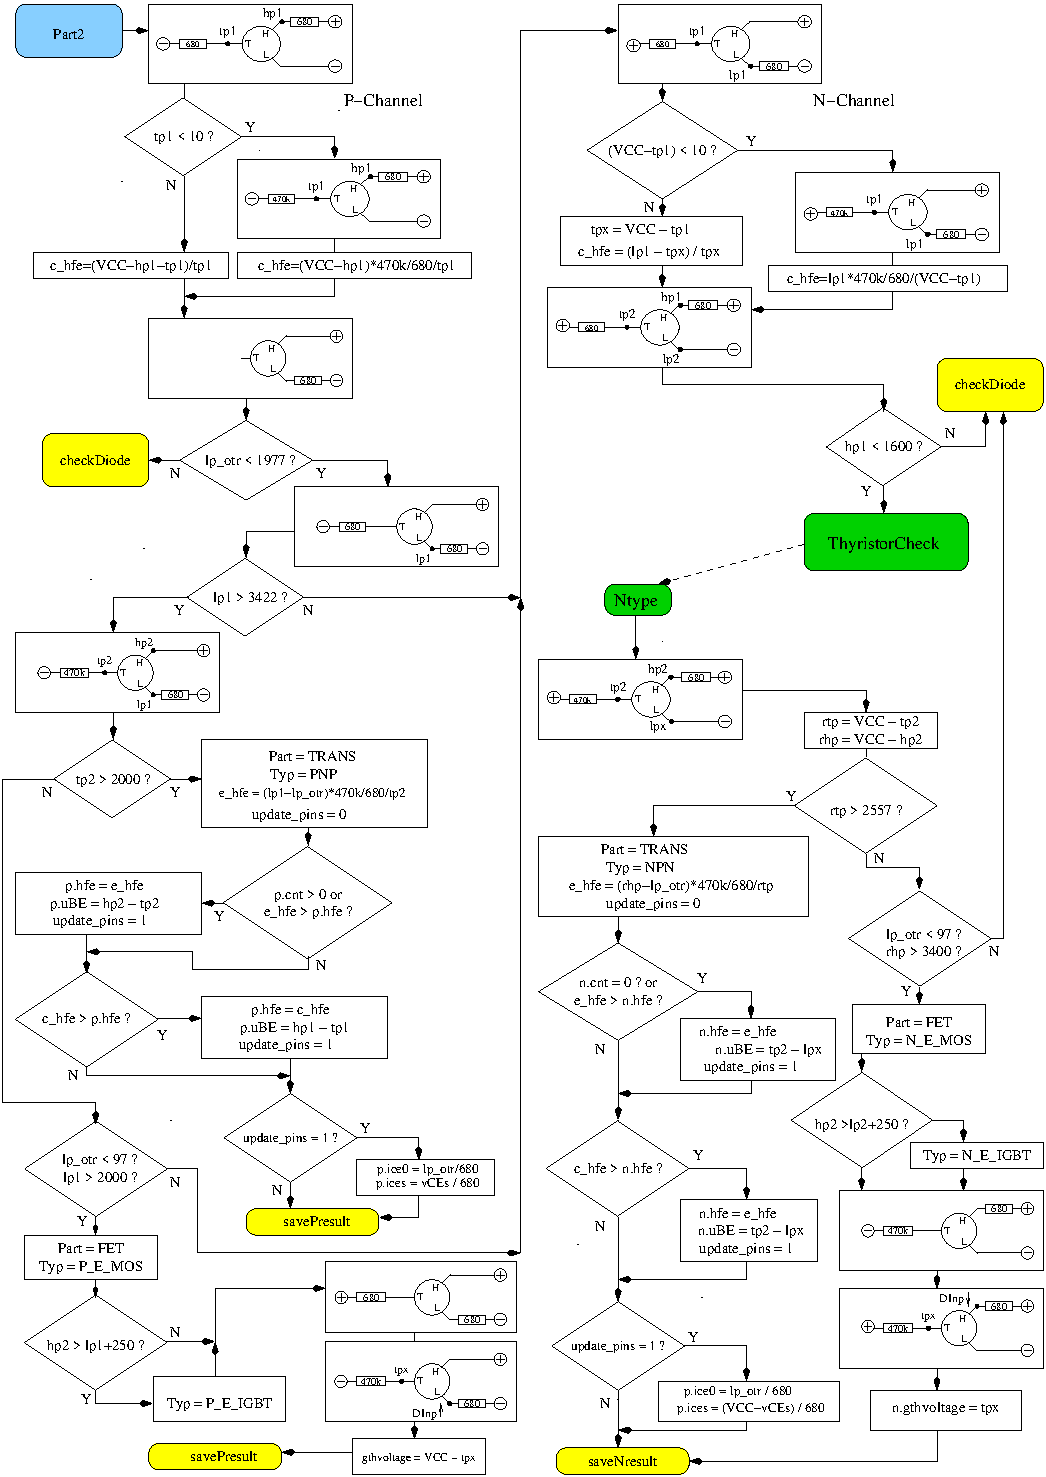
\includegraphics[width=.8\textwidth]{../FIG/CheckSemi2.pdf}
\caption{Flowchart transistor test Part 2, BJT and E-MOS}
\label{fig:ChkSemi2}
\end{figure}

\begin{figure}[H]
\centering
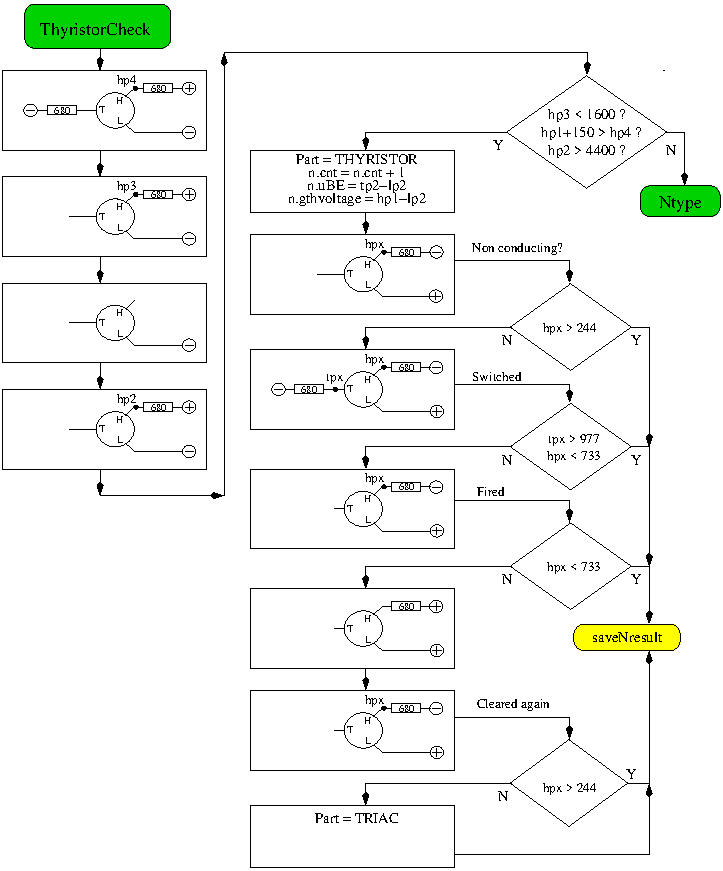
\includegraphics[width=.8\textwidth]{../FIG/CheckSemi3.pdf}
\caption{Flowchart transistor test Part 3, Thyristor and Triac}
\label{fig:ChkSemi3}
\end{figure}


\subsection{Measurement of Diodes}
\label{sec:diode}
If current is detected with the pre-tests, the behavior of the part will be checked to be a diode.
The flow voltage with the \(680~\Omega\) resistor must be between \(0.15~V\) and \(4.64~V\).
The flux voltage with the \(680~\Omega\) must be greater than 1.125 times the flux voltage with
the \(470~k\Omega\) resistor and sixteen times the flux voltage with the \(470~k\Omega\) must be
greater than the flux voltage with the \(680~\Omega\) resistor.
Additionally the afterward renewed measurement with the \(470~k\Omega\) resistor should not have a higher voltage than
the previous measurement with the \(680~\Omega\) resistor.
I hope, that this behavior identifies always a diode.
The identification of a diode by no current flow in the opposite direction is not
possible with a inverse parallel diode.
If only a single diode is detected, the residual current in reverse direction is measured with
the \(470~k\Omega\) resistor at \(5~V\). The resolution is about \(2~nA\).
If the residual current is greater as \(5.3~\mu A\) (voltage at
the \(470~k\Omega\) is more than \(2.5~V\)), the measurement is done with the \(680~\Omega\) instead.
Then the resolution is only about \(1~\mu A\).
Furthermore  the capacity in reverse direction is also measured for single diodes.

\subsection{Results of different measurements}
The following three tables shows results of different test probes 
with one ATmega8, a ATmega168 and a ATmega328 processor.
The measurement of the inverse capacity value for the double diode MBR4045PT is 
only possible with cooling. This will be caused by high residual current of this 40A diode.
Also the capacity value of the inverse base emitter diode of the germanium transistor AC128 can
only be measured with cooling.

\begin{table}[H]
  \begin{center}
    \begin{tabular}{| l | c | c | c |}
    \hline
           & Mega8@8MHz & Mega168 @8MHz & Mega328 @8MHz \\
 Diode Type  &                  &                  &                  \\
    \hline
    \hline
1N4148     & Diode, 715mV,        & Diode, 718mV,            & Diode, 715mV,           \\
           &               1pF    &               0pF, 2nA   &               1pF, 4nA  \\
    \hline
1N4150     & Diode, 665mV,        & Diode, 672mV,            & Diode, 666V,           \\
           &               1pF    &               1pF, 4nA   &              2pF, 6nA  \\
    \hline
BA157      & Diode, 619mV,        & Diode, 621V,              & Diode, 615mV,            \\
           &               19pF   &              17pF, 12nA   &               18pF, 12nA \\
    \hline
BY398      & Diode, 538mV,        & Diode, 541mV,             & Diode, 537mV,            \\
           &               16pF   &               14pF, 63nA  &               15pF, 63nA \\
    \hline
1N4007     & Diode, 650mV,        & Diode, 655mV,            & Diode, 650mV,           \\
           &               13pF   &               10pF, 6nA  &               13pF, 6nA \\
    \hline
LED green  & Diode, 1.96V, 5pF    & Diode, 1.95V, 4pF   & Diode, 1.95V, 4pF \\
    \hline
ZPD2,7     & 2xDi, 743mV, 2.53V   & 2xDi, 737mV, 2.52V  & 2xDi, 733mV, 2.51V \\
    \hline
BU508A B+E & Diode, 609mV,        & Diode, 611mV,                & Diode, 606mV,              \\
           &               5.15nF &               5.20nF, 0.39uA &               5.25nF, 0.4uA\\
    \hline
BU508A B+C & Diode, 582mV,        & Diode, 586mV,             & Diode, 587mV,            \\
           &               256pF  &               255pF, 21nA &               259pF, 19nA\\
    \hline
AC128 B+E  & Diode, 272mV,        & Diode, 277mV,              & Diode, 273mV,             \\
           &               0pF    &               0pF, 2.2uA   &               0pF, 2.3uA  \\
    \hline
AC128 B+E  &                      &                     & Diode, 349mV,               \\
cooled     &                      &                     &               140pF, 0.57uA \\
    \hline
MBR20100CT & 2xDi, 337mV, 337mV   & 2xDi, 338mV, 338mV  & 2xDi, 336mV, 335mV  \\
    \hline
MBR20100CT & Diode, 337mV,        & Diode, 339mV,             & Diode, 337mV,            \\
           &               345pF  &               351pF, 29nA &               350pF, 25nA\\
    \hline
MBR4045PT  & Diode, 243mV,        & Diode, 233mV,               & Diode, 235mV,              \\
cooled     &               1.80nF &               1.94nF, 1.7uA &               1.95nF, 1.8uA\\
    \hline
SK14       & Diode,    mV,        & Diode,    mV,               & Diode, 263mV,              \\
           &                  0pF &                   pF,    nA &               0pF, 0.57uA\\
    \hline
SK14       & Diode,    mV,        & Diode,    mV,               & Diode, 334mV,              \\
cooled     &                   nF &                   pF,    nA &               88pF, 4nA\\
    \hline
SF38G      & Diode, 519mV,        & Diode, 521mV,            & Diode, 516mV,            \\
           &               107pF  &               105pF, 2nA &               106pF, 2nA \\
    \hline
    \end{tabular}
  \end{center}
  \caption{measurement results of diode testing}
  \label{tab:diodes} 
\end{table}

\begin{table}[H]
  \begin{center}
    \begin{tabular}{| l | c | c | c | c | c |}
    \hline
 Transistor & Typ & Mega8           & Mega328        & Mega328         & Mega328 \\
    Type     &     & common-         &                & common-         & common- \\
            &     & collector      &                & collector       & emitter \\
    \hline
    \hline
BU508A      & NPN & B=9, 601mV      &  B=9, 597mV    &   B=9, 598mV    & B=4, 484mV \\
    \hline
2N3055      & NPN & B=20, 557mV     &  B=21, 550mV   &   B=21, 550mV   & B=6, 442mV \\
    \hline
BC639       & NPN & B=148, 636mV    &  B=172, 629mV  &   B=172, 629mV  & B=158, 605mV \\
    \hline
BC640       & PNP & B=226, 650mV    &  B=176, 609mV  &   B=171, 655mV  & B=177, 608mV \\
    \hline
BC517       & NPN & B=23.9k, 1.23V  &  B=24.8k, 1.22V&   B=25.1k, 1.22V & B=764, 1.23V \\
    \hline
BC516       & PNP & B=75.9k, 1.21V  &  B=76.2k, 1.20V&   B=76.2k, 1.20V & B=760, 1.23V \\
    \hline
BC546B      & NPN & B=285, 694mV    &  B=427, 687mV  &   B=427, 687mV   & B=369, 683mV \\
    \hline
BC556B      & PNP & B=304, 704mV    &  B=254, 668mV  &   B=235, 709mV   & B=255, 668mV \\
    \hline
AC128 (Ge.) & PNP & B=63, 191mV     &  B=59, 191mV   &   B=57, 193mV    & B=43, 117mV \\
    \hline
BUL38D      & NPNp & B=37, 627mV    &  B=41, 617mV  &   B=40, 624mV     & B=36, 562mV \\
parasitic   & PNPn & B=11, 654mV    &  B=81, 543mV  &   B=10, 656mV     & B=83, 541mV \\
    \hline
BRY55/200   & Thyrist. &  0.84V     &  0.81V         &   0.81V          &  0.82V \\
    \hline
MAC97A6     & Triac    &  0.92V     &  0.90V         &   0.90V          &  0.90V \\
    \hline
    \end{tabular}
  \end{center}
  \caption{measurement results of bipolar transistor testing}
  \label{tab:bipolar} 
\end{table}

Some results are very different to the earlier results of the software of Markus Frejek.
For example a darlington transistor BC517 has been measured by the older software
with a hFE of 797 instead of 77200 and a base emitter voltage of \(1438~mV\).
This will be caused by the additional measurement of current amplification with the
common collector circuit.
Also the new version shows the same low hFE result with the common emitter circiut,
as you can see in the last column of table~\ref{tab:bipolar}.
The base emitter voltage is measured by the older Version as separate diode test with \(1438~mV\).
Now the base emitter voltage is measured with the state of current amplification testing (\(1.20~V\)).
The BUL38D Transistor has a build in protection diode over the anode and cathode of the NPN transistor,
by what a parasitical PNP transistor with swapped Base - Collector connection is build.
With software revision 1.10k both transistors are detected and marked
with a appended p.
The right transistor will be found with comparation of the gate - emitter junction capacitance.
It is assumed, that the right transistor has the higher junction capacitance.
If you hold down the start key during the output of the measurement result, the parameter of
the parasitical transistor are shown. With the label PNPn the existance of another transistor will be marked.
The parasitical transistor structure is build only by integration of the protection diode nearby
the transistor within the same material, not with a external diode.

The following table~\ref{tab:germanium} shows the measurement results for germanium transistors, which are extra problematic
to measure because of the temperatur dependent and high residual collector current.
The results of the original version of Markus F. and the results of the actual 1.10k version are
compared together. The 1.10k version for a ATmega328 measures the current amplification factor with
common collector and common emitter circuit with respect to the collector residual current,
the higher result will be shown.
The collector residual current is not respected by earlier versions.

\begin{table}[H]
  \begin{center}
    \begin{tabular}{| l | c | c | c |}
    \hline
 Transistor & Mega8@1MHz          & Mega168 @8MHz       & Mega328 @8MHz    \\
    Type    & Original Version    & Version 1.10k       & Version 1.10k  \\
            & Markus F.           &                     &        \\
    \hline
    \hline
AC128       & PNP, B=52, 279mV    & PNP, B=59, 184mV    & PNP, B=59, 191mV    \\
    \hline
AC116-65    & PNP, B=505, 378mV   & PNP, B=72, 146mV    & PNP, B=72, 149mV    \\
    \hline
AC116-145   & PNP, B=485, 294mV   & PNP, B=146, 161mV    & PNP, B=146, 163mV   \\
    \hline
AC176-65    & NPN, B=98, 235mV    & NPN, B=58, 94mV    & NPN, B=56, 96mV     \\
    \hline
GC122       & PNP, B=84, 368mV    & PNP, B=55, 117mV    & PNP, B=56, 117mV    \\
    \hline
GC301       & PNP, B=48, 289mV    & PNP, B=39, 184mV    & PNP, B=39, 188mV    \\
    \hline
AD161       & NPN, B=360, 230mV   & NPN, B=296, 126mV   & NPN, B=298, 128mV    \\
    \hline
AD162       & PNP, B=2127, 280mV  & PNP, B=89, 107mV    & PNP, B=89, 107mV    \\
    \hline
    \end{tabular}
  \end{center}
  \caption{Measurement results of bipolar junction germanium transistors}
  \label{tab:germanium}
\end{table}

In the table~\ref{tab:mos} the results of some field-effect transistor measurements are shown.
One measured parameters of the E-type MOS types is the gate-source voltage, by which the
digital input of the ATmega connected to the \(680~\Omega\) drain resistor
changes the state.
For very fast change of the gate voltage due to a small gate capacity, the detected voltage is
slightly inaccurate.
With the BS250 the Voltage changes from \(2.6~V\) to \(2.5~V\), if you connect a additional
\(10~nF\) capacitor to the gate-source.

Another imeasured parameter is the gate capacity value.
The gate capacity is measured by switching the source and drain pin to the GND potential.
The available \(5V\) gate voltage of the tester is unsufficient to generate some collector current
with some IGBTs. This will prevent the correct detection.
Only the collector-emitter protection diode is detected then in most cases.
A Battery with about \(3V\) connected to the gate pin can solve this problem with the detection.
The other pole of the battery should be connected to a test pin (TP) of the tester instead of the gate connection.
With the right polarity of the battery the tester should detect the IGBT now.
The shown gate-emitter switching voltage must be increased by the value of the battery voltage
to get the right switching voltage.

For JFET transistors often the characteristic current Idss is specified,
the current in the drain when the gate-source voltage is \(0~V\).
Here, however, the current is given by a \(680~\Omega\) load resistance at the source side
of the JFET.
The load resistor generates a reverse voltage Vgs,
which is also shown.
With a \(470k\Omega\) load resistor at the source side of the JFET the Source-Drain current will
be nearly zero. With this circuit we can get the Gate-Source Cutoff voltage Vgs\_off exactly enough,
if the voltage remain below \(5V\).
With this two operating points we can estimate the current Igss with the nearly quadratic characteristic
curve of the current.
If the estimated current Idss stay below \(40mA\), a additional measurement is done without
a additional resistor at the source pin.
With the measured voltage at the source pin we can compute a additional current value.
Now we can compute a better estimated current Idss with this higher current valued, the gate-source voltage
and with the known quadratic current curve, if the value of \(40mA\) is not exeeded.
Due to the symmetrical design of the JFET transistors, the drain and source can not be distinguished.


\begin{table}[H]
  \begin{center}
    \begin{tabular}{| l | c | c | c | c |}
    \hline
             &         & Mega8@8MHz       & Mega168 @8MHz    & Mega328 @8MHz \\
 Transistor  & Type    &                  &                  &               \\
    \hline
    \hline
ZVNL120A     & N-E-MOS & D, 1.6V, 147pF   & D, 1.5V,141pF    & D, 1.5V, 140pF \\
    \hline
IRF530N      & N-E-MOS & D, 3.6V, 1.55nF  & D, 3.6V, 1.54nF  & D, 3.6V, 1.54nF \\
    \hline
BS170        & N-E-MOS & D, 2.6V, 78pF    & D, 2.6V, 68pF    & D, 2.6V, 68pF \\
    \hline
IRL3803      & N-E-MOS & D, 2.3V, 9.81nF  & D, 2.3V, 9.71nF  & D, 2.3V, 9.74nF \\
    \hline
IRFU120N     & N-E-MOS & D, 4.2V, 909pF   & D, 4.2V, 913pF   & D, 4.2V, 911pF \\
    \hline
BUZ71A       & N-E-MOS & D, 3.2V, 714pF   & D, 3.2V, 708pF   & D, 3.2V, 705pF \\
    \hline
ZVP2106A     & P-E-MOS & D, 3.2V, 122pF   & D, 3.2V,115pF    & D, 3.2V, 116pF \\
    \hline
IRF5305      & P-E-MOS & D, 3.6V, 2.22nF  & D, 3.6V, 2.22nF  & D, 3.6V, 2.22nF \\
    \hline
BS250        & P-E-MOS & D, 2.6V, 53pF    & D, 2.6V, 43pF    & D, 2.6V, 44pF \\
    \hline
IRFU9024     & P-E-MOS & D, 3.5V, 937pF   & D, 3.6V, 945pF   & D, 3.5V, 933pF \\
    \hline
J310         & N-JFET  & 3.1mA Vgs=2.2V   & 3.1mA Vgs=2.2V   & 3.1mA Vgs=2.2V \\
Idss=24-60mA &         &                  &                  & Idss=35mA      \\
    \hline
2N5459       & N-JFET  & 2.1mA Vgs=1.5V   & 2.1mA Vgs=1.5V   & 2.1mA Vgs=1.5V \\
Idss=4-16mA &          &                  &                  & Idss=8.2mA     \\
    \hline
BF256C       & N-JFET  & 3.4mA Vgs=2.4V   & 3.4mA Vgs=2.4V   & 3.4mA Vgs=2.4V \\
Idss=11-18mA &         &                  &                  & Idss=14mA      \\
    \hline
BF245A       & N-JFET  & 1.1mA Vgs=.75V   & 1.1mA Vgs=0.75V  & 1.1mA Vgs=0.75V \\
Idss=2-6mA   &         &                  &                  & Idss=3.6mA      \\
    \hline
BF245B       & N-JFET  & 2.5mA Vgs=1.7V   & 2.5mA Vgs=1.7V   & 2.5mA Vgs=1.7V \\
Idss=6-15mA  &         &                  &                  & Idss=10mA      \\
    \hline
BF245C       & N-JFET  & 3.9mA Vgs=2.7V   & 3.9mA Vgs=2.7V   & 3.9mA Vgs=2.7V \\
Idss=12-25mA &         &                  &                  & Idss=17mA    \\
    \hline
J175        & P-JFET   & 3.2mA Vgs=2.2V   & 3.2mA Vgs=2.2V   & 3.2mA Vgs=2.2V \\
Idss=7-60mA &          &                  &                  & Idss=26mA      \\
    \hline
2N5460      & P-JFET   & 0.78mA Vgs=0.54V & 0.77mA Vgs=0.54V & 0.78mA Vgs=0.54V \\
Idss=1-5mA  &          &                  &                  & Idss=2.6mA       \\
    \hline
BSS139      & N-D-MOS  & 1.7mA Vgs=1.2V  & D, 1.7mA Vgs=1.2V & D, 1.7mA Vgs=1.2V \\
    \hline
BSS169      & N-D-MOS  & 2.6mA Vgs=1.8V  & D, 2.6mA Vgs=1.8V & D, 2.6mA Vgs=1.8V \\
    \hline
GP07N120    & N-E-IGBT & C=3.81nF Vt=4.2V & C=3.76nF Vt=4.2V & C=3.74nF Vt=4.2V \\
    \hline
IRG4PC30    & N-E-IGBT &                  &                  & C=2.22nF         \\
with Bat.   &          &                  &                  & Vt=2.0V+3.2V \\
    \hline
    \end{tabular}
  \end{center}
  \caption{measurement results of MOS transistor testing}
  \label{tab:mos} 
\end{table}
